\documentclass{amsart}
\usepackage{graphicx}
\graphicspath{{./}}
\usepackage{hyperref}
\usepackage{csvsimple}
\usepackage{longtable}
\usepackage{lscape}
\usepackage{epigraph}
\title{Ethnicity Effects on Hard Work or Luck in Success}
\author{Zulfikar Moinuddin Ahmed}
\date{\today}
\begin{document}
\maketitle

\section{The Curves}

This is ethnicity-factored Q110.

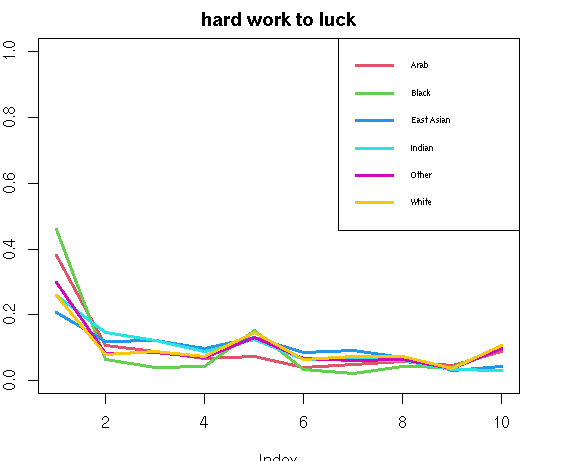
\includegraphics[scale=0.8]{ethhardworkluck.jpeg}

\section{Elementary Inferences}

The curves are quite close to each other.  It is amusing to see that on the right tail highest are white people which tells us that various 'myths of lazy natives' are wrong.  Those sorts of myths were propaganda for colonial projects and were always false.  

\subsection{Slow Decay for All Ethnicities}

You can see visually that these are exponentially decreasing with noise, so 'success is due to hard work' is higher for all ethnicities but the decay is slow as well, so there are substantial proportions who all think that success is more due to luck.

\section{Ethnicity Effects}
% latex table generated in R 4.0.3 by xtable 1.8-4 package
% Fri May 14 16:27:09 2021
\begin{table}[ht]
\centering
\begin{tabular}{rlr}
  \hline
 & eth & explained \\ 
  \hline
1 & Arab & 4.42 \\ 
  2 & Black & 11.98 \\ 
  3 & East Asian & 12.72 \\ 
  4 & Indian & 5.84 \\ 
  5 & Other & 0.62 \\ 
  6 & White & 3.43 \\ 
   \hline
\end{tabular}
\end{table}

The sober assessment is that the effects are around 10\% or less and negligible from ethnicity.

Both qualitatively and quantitatively, there is an slow exponential decrease from 'hard work' to 'luck' across all ethnicities.

\section{Exponential Model Fits}

% latex table generated in R 4.0.3 by xtable 1.8-4 package
% Fri May 14 19:01:00 2021
\begin{table}[ht]
\centering
\begin{tabular}{rlrr}
  \hline
 & eth & lambda & rsq \\ 
  \hline
1 & Arab & 0.14 & 0.41 \\ 
  2 & Black & 0.12 & 0.17 \\ 
  3 & East Asian & 0.16 & 0.80 \\ 
  4 & Indian & 0.21 & 0.91 \\ 
  5 & Other & 0.11 & 0.37 \\ 
  6 & White & 0.09 & 0.28 \\ 
   \hline
\end{tabular}
\end{table}

These are not extremely tight fits but they are reasonable.  We obtain mean $\lambda=0.138$ and mean $R^2=0.49$.

\section{Sufficient evidence For Exponential Inference}

The fits above provide us with sufficient evidence to consider the ramifications of an exact exponential distribution for hard work to luck as convictions of people.  The exponential parameter has standard deviation $\sigma(\lambda) = 0.0415$.  

We can model the random person picked from the human race as having preference from $Exp(0.138)$ on hard work to luck for success axis.

Note that the small variance $\sigma(\lambda)=0.0415$ is another indicator of the small influence of ethnicity; the exponential decay changes by a little bit based on ethnicity but retains exponential.

\end{document}